\documentclass{article}
\usepackage[T1]{fontenc}
\usepackage{lmodern}
\usepackage{graphicx}
\usepackage{amsmath,amssymb}
\usepackage[a4paper,margin=2cm]{geometry}
\usepackage[absolute,overlay]{textpos}
\setlength{\TPHorizModule}{1mm}
\setlength{\TPVertModule}{1mm}
\usepackage[indonesian]{babel}
\usepackage{hyperref}
\setlength{\emergencystretch}{2em}
% unit: Halaman 42

\begin{document}

% === Halaman 42 (llm) ===

\section*{Citra Lenna}

\vspace{10mm}

\begin{center}
\begin{tabular}{ccc}
True color image & Grayscale image & Bimary image \\
(24-bit) & (8-bit) & (1-bit) \\
\end{tabular}
\end{center}

% deskripsi: Contoh citra Lenna dalam tiga format berbeda: warna asli (24-bit), skala abu-abu (8-bit), dan biner (1-bit).
% bbox normalisasi: [0.1200, 0.2500, 0.8600, 0.6200]
\begin{textblock*}{155.40mm}(25.20mm,74.25mm)
\noindent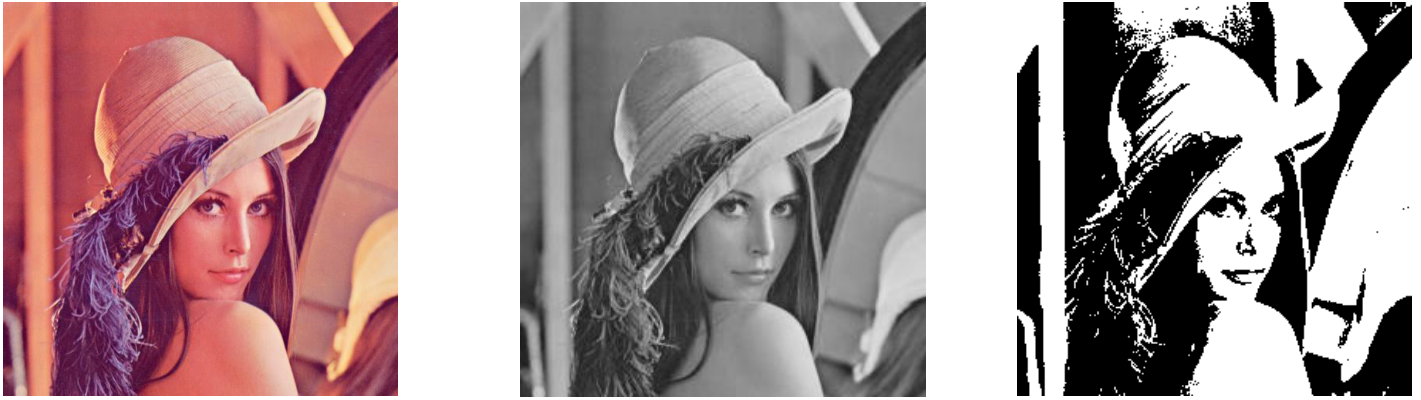
\includegraphics[width=155.40mm,height=109.89mm]{../../images/llm/page_042_img_01.png}%
\end{textblock*}

\end{document}
